% (c) 2014 Daniele Masini - d.masini.it@gmail.com
\chapter{Il teorema di Bayes}

\section{Dalla tavola statistica alla probabilità}

Consideriamo la seguente tabella che rappresenta la popolazione
residente in Italia per classi di età e sesso al primo gennaio 2009
(migliaia di persone).

\begin{center}
\begin{tabular}{lccccc}
& $ A_1 $
& $ A_2 $
& $ A_3 $
& $ A_4 $
& \\

& $ 0\le \text{età}<20 $
& $ 20\le \text{età}<40 $
& $ 40\le \text{età}<60 $
& $ \text{età}\ge 60 $
& Totale\\

M = Maschio & $ \np{5867} $ & $ \np{8014} $ & $ \np{8473} $ & $ \np{6798} $ & $ \np{29152} $ \\
F = Femmina & $ \np{5541} $ & $ \np{7845} $ & $ \np{8649} $ & $ \np{8857} $ & $ \np{30892} $ \\

Totale & $ \np{11408} $ & $ \np{15859} $ & $ \np{17122} $ & $ \np{15655} $ & $ \np{60044} $ %\\\hline
\end{tabular}
\end{center}

L'esperimento in questo caso è costituito da una
classificazione dei residenti secondo il sesso: (Maschi e Femmine) e
classi di età ($ A_1 $, $ A_2 $, $ A_3 $, $ A_4 $).

I valori assoluti presenti
all'interno delle celle rappresentano le persone che
hanno in comune  due caratteri, cioè:

\[M\cap A_{1}=\np{5867}\text{, }F\cap A_{1}=\np{5541}\text{, }\ldots M\cap A_{4}=\np{6798}\text{, }F\cap A_{4}=\np{8857}.\]

In questo caso gli eventi elementari sono rappresentati dalle
intersezione delle modalità dei due caratteri:
\[\Omega=\{(M,A_{1})\text{, }(M,A_{2})\text{, }(M,A_{3})\text{, }(M,A_{4})\text{, }(F,A_{1})\text{, }(F,A_{2})\text{, }(F,A_{3})\text{, }(F,A_{4})\}.\]

Dato che il campione analizzato è l'intera popolazione
italiana residente possono essere l'informazione di base per il calcolo della
probabilità.

Per far questo passiamo alle frequenze relative. 
Notiamo innanzitutto che, essendo eventi elementari, questi eventi sono tra loro incompatibili ed esaustivi, infatti indicate con $ (M,A_{i}) $ e $ (M,A_{j}) $ due generiche celle con $ i\neq j $ abbiamo:
\[(M,A_{i})\cap(M,A_{j})=\emptyset~\text{ e }\sum_{n=1}^4 (M,A_{n})\cup(F,A_{n})=\Omega.\]

Il calcolo delle frequenze relative è dato dal valore assoluto di ogni cella diviso per il valore assoluto del totale della popolazione. Così $M\cap A_1=\frac{\np{5867}}{\np{60044}}=\np{0,098}$, $F\cap A_2=\frac{\np{7845}}{\np{60044}}=\np{0,131}$, $F\cap A_4=\frac{\np{8857}}{\np{60044}}=\np{0,148}$.
Tutte le frequenze relative sono indicate nella tabella seguente.

\begin{center}
\begin{tabular}{lccccc}
& $ A_1 $
& $ A_2 $
& $ A_3 $
& $ A_4 $
& \\

& $ 0\le \text{età}<20 $
& $ 20\le \text{età}<40 $
& $ 40\le \text{età}<60 $
& $ \text{età}\ge 60 $
& Totale\\

M = Maschio & $ \np{0,098} $ & $ \np{0,133} $ & $ \np{0,141} $ & $ \np{0,113} $ & $ \np{0,485} $ \\
F = Femmina & $ \np{0,092} $ & $ \np{0,131} $ & $ \np{0,144} $ & $ \np{0,148} $ & $ \np{0,515} $ \\

Totale & $ \np{0,190} $ & $ \np{0,264} $ & $ \np{0,285} $ & $ \np{0,261} $ & $ \np{1,000} $ %\\\hline
\end{tabular}
\end{center}

Aiutiamoci con i diagrammi di Venn per analizzare il significato dei
totali di riga e di colonna. Il grafico si riferisce al
totale della prima riga e della prima colonna: 
\[\begin{array}{l}{\text{prima riga: }\np{0,098}+\np{0,133}+\np{0,141}+\np{0,113}=\np{0,485}}\\{\text{prima colonna: }\np{0,098}+\np{0,092}=\np{0,190}.}\end{array}\]
\begin{center}
 % (c) 2012 Dimitrios Vrettos - d.vrettos@gmail.com
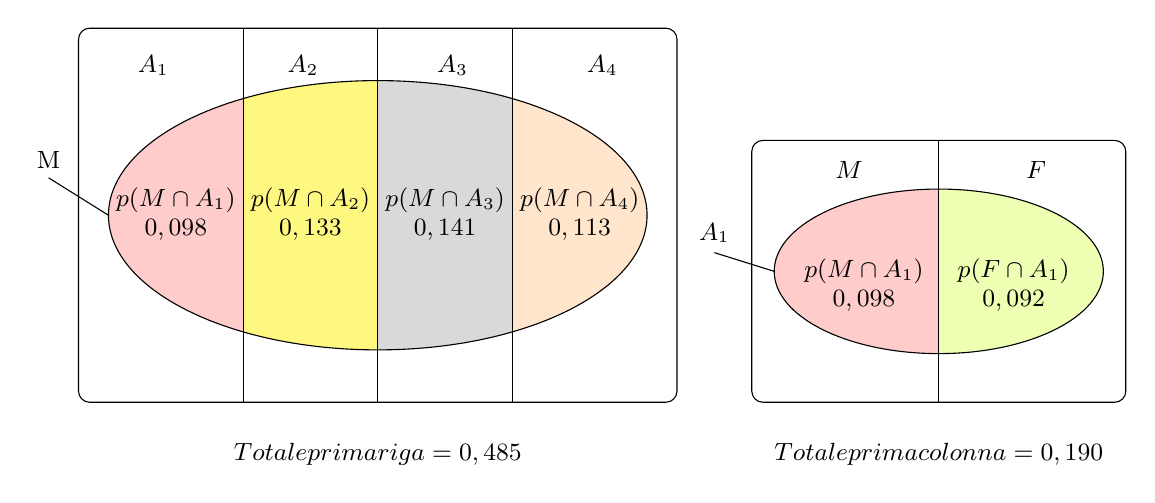
\begin{tikzpicture}[x=2cm,font=\small,scale=.95]
\def\firstcircle{(1.5,2.5) circle (1.8)}
\def\firstrett {(-.5,0) rectangle (1.1,5)}
\def\secrett {(.6,0) rectangle (2,5)}
\def\thirdrett {(1.5,0) rectangle (2.9,5)}
\def\fourrett {(2.4,0) rectangle (4,5)}
\def\seccircle{(5.25,1.75) circle (1.1)}
\def\fiftrett {(6.5,0) rectangle (2,5)}
\def\sexrett {(5.25,0) rectangle (2,3.5)}

\draw[rounded corners] (-.5,0) rectangle (3.5,5);
\begin{scope}
\clip \firstcircle;
\fill[red!20]\firstrett;
\clip \firstcircle;
\fill[yellow!50]\secrett;
\clip \firstcircle;
\fill[gray!30]\thirdrett;
\clip \firstcircle;
\fill[orange!20]\fourrett;
\end{scope}

\draw\firstcircle;

\draw (.6,5)--(.6,0);\draw(1.5,5)--(1.5,0);\draw(2.4,5)--(2.4,0);
\draw(-.7,3)--(-.3,2.5);
\node [above]at (-.7,3) {M};
\node at (0,4.5){$A_1$};\node at (1,4.5){$A_2$};\node at (2,4.5){$A_3$};\node at (3,4.5){$A_4$};
\node at (.15,2.7){$p(M\cap A_1)$};\node at (.15,2.3){$0,098$};
\node at (1.05,2.7){$p(M\cap A_2)$};\node at (1.05,2.3){$0,133$};
\node at (1.95,2.7){$p(M\cap A_3)$};\node at (1.95,2.3){$0,141$};
\node at (2.85,2.7){$p(M\cap A_4)$};\node at (2.85,2.3){$0,113$};
\node at (1.5,-.7){$\text{Totale prima riga}=0,485$};

\draw[rounded corners] (4,0) rectangle (6.5,3.5);

\begin{scope}
\clip \seccircle;
\fill[lime!30]\fiftrett;
\clip \seccircle;
\fill[red!20]\sexrett;
\end{scope}

\draw\seccircle;
\draw(5.25,3.5)--(5.25,0);
\node[above] at (3.75,2){$A_1$};
\draw(3.75,2)--(4.15,1.75);
\node at (4.75,1.75){$p(M\cap A_1)$};\node at (4.75,1.35){$0,098$};
\node at (5.75,1.75){$p(F\cap A_1)$};\node at (5.75,1.35){$0,092$};
\node at (4.65,3.1){$M$};\node at (5.9,3.1){$F$};
\node at (5.25,-.7){$\text{Totale prima colonna}=0,190$};

\end{tikzpicture}

\end{center}

Dato che gli
eventi intersezione sono tra loro incompatibili i totali di riga e di
colonna, detti anche \emph{totali marginali}, rappresentano le probabilità delle
modalità semplici Maschio e Femmina e  $ A_1 $, $ A_2 $, $ A_3 $, $ A_4 $ relative alle
classi di età.

Ma c'è di più. Nella tabella così strutturata abbiamo a
disposizione sia la probabilità dell'intersezione
delle modalità degli eventi, che la probabilità degli eventi stessi.
Possiamo calcolare così anche le probabilità condizionate con la formula studiata nel capitolo sulla probabilità a pagina \pageref{pr_cond}:
\begin{equation}
\label{eqn:bayes}
p(B/A)=\frac{p(A\cap B)}{p(A)}.
\end{equation}
Le condizioni per trattare la probabilità come negli esempi precedenti
sono che gli eventi presenti nelle righe e nelle colonne della tabella,
siano eventi \emph{esaustivi} e \emph{incompatibili}, in altre parole devono
rappresentare un insieme di eventi elementari. Questo è sempre
possibile dati due eventi elementari  $A$  e  $B$  considerando gli
eventi complementari  $\overline{{A}}$  e  $\overline{{B}}$.

\begin{exrig}
\begin{esempio}
Il daltonismo è una malattia genetica collegata al sesso e si
osserva più frequentemente nei maschi che nelle femmine. Le frequenze
relative della seguente tabella, osservate su un campione molto elevato
di popolazione, possono essere usate come probabilità.
\begin{center}
\begin{tabular}{lccc}
& p(Daltonico) & p(Non Daltonico) & Totale\\
p(Maschio)& $ 8,1\% $ & $ 45,0\% $ & $ 53,1\% $ \\
p(Femmina)& $ 0,5\% $ & $ 46,4\% $ & $ 46,9\% $ \\
Totale & $ 8,6\% $ & $ 91,4\% $ & $ 100\% $\\
\end{tabular}
\end{center}
$ P(D) $ indica la probabilità di essere daltonico, questa probabilità si
legge nel totale marginale della prima colonna ed è pari a $ 8,6\% $. La
probabilità di non essere daltonico $ P(ND) $ è data dal totale marginale
della seconda colonna e rappresenta la probabilità complementare del
primo evento pari a  $ 91,4\% $.

I totali marginali di riga indicano la probabilità di essere maschio
pari al $ 53,1\% $ e la probabilità di essere femmina pari al $ 46,9\% $.

Nella tabella abbiamo quindi tutte le probabilità che ci consentono di
calcolare le probabilità condizionate. In particolare:
\begin{itemize*}
\item Probabilità condizionata che un maschio sia daltonico, incidenza
del daltonismo per i maschi
\[p(D/M)=\frac{p(D\cap M)}{p(M)}=\frac{8,1\%}{53,1\%}=15,3\%;\]

\item Probabilità condizionata che una femmina sia daltonica, incidenza
del daltonismo per le femmine
\[p(D/F)=\frac{P(D\cap F)}{p(F)}=\frac{0,5\%}{46,9\%}=1,1\%;\] 

\item Probabilità condizionata che un daltonico sia maschio, incidenza
dei maschi per il daltonismo
\[p(M/D)=\frac{p(D\cap M)}{p(D)}=\frac{8,1\%}{8,6\%}=94,2\%;\]

\item Probabilità condizionata che un daltonico sia femmina, incidenza
delle femmine per il daltonismo
\[p(F/D)=\frac{p(D\cap F)}{p(D)}=\frac{0,5\%}{8,6\%}=5,8\%.\]
\end{itemize*}
\end{esempio}

\begin{esempio}
Un test diagnostico è qualsiasi procedimento che sappia individuare
se un individuo è soggetto a una determinata malattia cioè se è malato $ M^+ $ o
sano $ M^- $. Un test può dare esito positivo (cioè indicare che
l'individuo è malato) $ T^+ $ o negativo (indicare che un
individuo è sano) $ T^- $. Si sa però che le indicazioni dei più comuni
test non sono del tutto sicure, può accadere che un individuo risultato
positivo al test sia invece sano e viceversa. Quindi è necessario dare
una valutazione delle caratteristiche di un test diagnostico.

Immaginiamo che un determinato test diagnostico sia sotto
sperimentazione e che i risultati ottenuti siano indicati dalla
seguente tabella
\begin{center}
\begin{tabular}{lccc}
& $\text{Positivo}=T^+$ & $\text{Negativo}=T^-$ & Totale\\
$\text{Malato}=M^+$& $ \np{4120} $ & $ \np{512} $ & $ \np{4632} $ \\
$\text{Sano}=M^-$& $ \np{1560} $ & $ \np{4322} $ & $ \np{5882} $ \\
Totale & $ \np{5680} $ & $ \np{4834} $ & $ \np{10514} $\\
\end{tabular}
\end{center}
Dato che la popolazione coinvolta è considerata significativa, possiamo
passare alle frequenze  relative e considerarle come una valutazione
della probabilità.
\begin{center}
\begin{tabular}{lccc}
& $\text{Positivo}=T^+$ & $\text{Negativo}=T^-$ & Totale\\
$\text{Malato}=M^+$& $ 39,2\% $ & $ 4,9\% $ & $ 44,1\% $ \\
$\text{Sano}=M^-$& $ 14,8\% $ & $ 41,1\% $ & $ 55,9\% $ \\
Totale & $ 54,0\% $ & $ 46,0\% $ & $ 100\% $\\
\end{tabular}
\end{center}
In ogni cella leggiamo la probabilità dell'intersezione
dei due caratteri, mentre nei totali marginali la probabilità di essere
malato e sano (totali di riga) e la probabilità che il test sia
risultato positivo o negativo (totali di colonna).

\begin{description*}
\item  $p(M^{+}\cap T^{+})=39,2\%$ \quad probabilità che un malato sia positivo al test (vero positivo);
\item  $p(M^{+{}}\cap T^{-})=4,9\%$ \quad probabilità che un malato sia negativo al test (falso negativo);
\item  $p(M^{-}\cap T^{+})=14,8\%$ \quad probabilità che un sano sia positivo al test (falso positivo);
\item  $p(M^{-}\cap T^{-})=41,1\%$ \quad probabilità che un sano sia negativo al test (vero negativo);
\item  $p(M^{+})=44,1\%$ \quad probabilità di essere malato;
\item  $p(M^{-{}})=55,9\%$ \quad probabilità di essere sano;
\item  $p(T^{+})=54,0\%$ \quad probabilità che il test sia positivo;
\item  $p(T^{-})=46,0\%$ \quad probabilità che il test sia positivo.
\end{description*}
Questo è quello che ci dicono i dati grezzi della precedente tabella. Ma
con alcuni semplici calcoli si possono calcolare le probabilità
condizionate, che ci danno informazioni più rilevanti. In particolare:
\begin{itemize*}
\item \emph{sensibilità del test} cioè la probabilità che un malato sia positivo  
\[p(T^{+}/M^{+})=\frac{p(T^{+}\cap M^{+})}{M^{+}}=\frac{39,2\%}{44,1\%}=88,9\%;\]

\item \emph{specificità del test} cioè la probabilità che un sano sia negativo 
\[p(T^{-}/M^{-})=\frac{p(T^{-{}}\cap M^{-})}{M^{-}}=\frac{41,1\%}{55,9\%}=73,5\%;\]

\item \emph{valore predittivo del test} cioè la probabilità che un positivo sia malato
\[p(M^{+}/T^{+})=\frac{p(T^{+}\cap M^{+})}{T^{+}}=\frac{39,2\%}{54,0\%}=72,6\%.\]
\end{itemize*}
\end{esempio}
\end{exrig}

\section{Teorema di Bayes}
Il teorema di Bayes fornisce un metodo che consente di modificare
l'opinione iniziale sul verificarsi di un evento (espressa sotto forma
di probabilità a priori) sulla base delle informazioni fornite
dall'esperienza che permettono di formulare nuove probabilità dette
probabilità a posteriori.

\begin{exrig}
\begin{esempio}
Supponiamo che un paziente vada a farsi visitare da un medico per la
prima volta.

Già prima di effettuare la visita il medico ha un'idea delle possibili
malattie da cui potrebbe essere affetto: sa che molti dei suoi pazienti
hanno disturbi di poco conto (evento $ H_1 $), alcuni hanno disturbi più
gravi (evento $ H_2 $), altri ancora malattie rare (evento $ H_3 $).

A questo punto il medico effettuerà la visita, sottoporrà il paziente ad
una serie di analisi cliniche ed otterrà il quadro dei sintomi: potrà
adesso formulare una diagnosi sul paziente.

Vediamo che cosa rappresenta tutto ciò in termini di probabilità.

Indichiamo con $ H_1 $, $ H_2 $ ed $ H_3 $ le tre tipologie di malattia in ordine di
rarità: sulla base delle informazioni che il medico ha in relazione ai
propri pazienti può associare ad ognuno di questi eventi una
probabilità a priori $ p(H_i) $.

In funzione della sintomatologia riscontrata (rappresentata dall'evento
$ E $) si possono determinare sulla base delle statistiche ufficiali a
livello nazionale le probabilità condizionate $ p(E/H_i) $ che rappresentano
le probabilità che si manifestino tali sintomi se un paziente è affetto
da una delle tre tipologie di malattia in esame.

Ciò che ci interessa è ricavare le probabilità a posteriori $ p(H_i/E) $, che
rappresentano le probabilità che il paziente abbia contratto una delle
tre malattie, sapendo che presenta i sintomi rappresentati da $ E $. Su
questa base si formulerà la diagnosi.

Si conoscono o si possono conoscere le seguenti probabilità:

Probabilità sulla tipologia di malattia fornita
dall'esperienza del medico:
\[p(H_{1})=0,65;\quad p(H_{2})=0,30;\quad p(H_{3})=0,05.\]

Probabilità dei sintomi evidenziati dal paziente condizionate alla
gravità della malattia desunte dalle statistiche ufficiali: 
\[p(E/H_{1})=0,20;\quad p(E/H_{2})=0,60;\quad p(E/H_{3})=0,70 \]

La situazione può essere rappresentata con un Diagramma di Venn:
\begin{center}
 % (c) 2012 Dimitrios Vrettos - d.vrettos@gmail.com
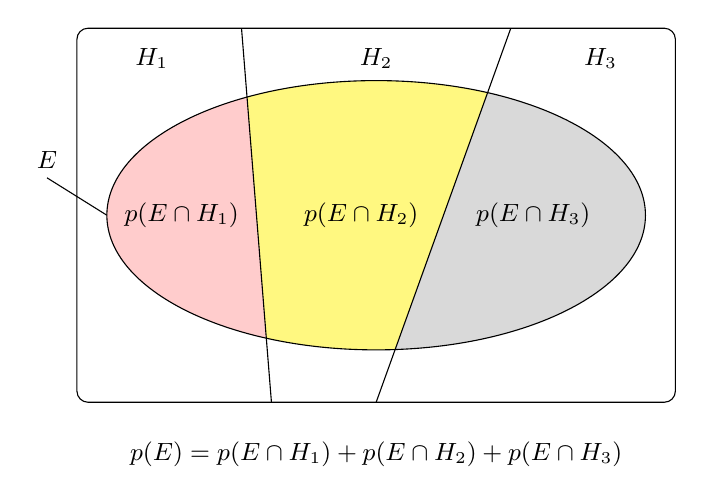
\begin{tikzpicture}[x=2cm,font=\small,scale=.95]
\def\firstcircle{(1.5,2.5) circle (1.8)}
\def\firstrett {(-.5,0) -- (-5,5) -- (.6,5) -- (.8,0) -- cycle}
\def\secrett {(.8,0) -- (.6,5) -- (2.4,5) -- (1.5,0) -- cycle}
\def\thirdrett {(1.5,0) -- (2.4,5) -- (4,5) -- (4,0) -- cycle}

\draw[rounded corners] (-.5,0) rectangle (3.5,5);
\begin{scope}
\clip \firstcircle;
\fill[red!20]\firstrett;
\clip \firstcircle;
\fill[yellow!50]\secrett;
\clip \firstcircle;
\fill[gray!30]\thirdrett;
\end{scope}

\draw\firstcircle;

\draw (.6,5)--(.8,0);\draw(2.4,5)--(1.5,0);
\draw(-.7,3)--(-.3,2.5);
\node [above]at (-.7,3) {$E$};
\node at (0,4.6){$H_1$};\node at (1.5,4.6){$H_2$};\node at (3,4.6){$H_3$};
\node at (.2,2.5){$p(E\cap H_1)$};
\node at (1.4,2.5){$p(E\cap H_2)$};
\node at (2.55,2.5){$p(E\cap H_3)$};
\node at (1.5,-.7){$p(E)=p(E\cap H_1)+p(E\cap H_2)+p(E\cap H_3)$};
\end{tikzpicture}

\end{center}

Essendo $ H_1 $ , $ H_2 $ e $ H_3 $ eventi incompatibili ed esaustivi, l'evento $ E $ può
essere visto come unione dei tre eventi disgiunti:  $E\cap H_{1}$, $E\cap H_{2}$ e $E\cap H_{3}$ 
Quindi\[p(E)=p(E\cap H_{1})+p(E\cap H_{2})+p(E\cap H_{3}).\]

Dall'equazione~\eqref{eqn:bayes} otteniamo $ p(A\cap B)=p(B/A)\cdot{p(A)} $ quindi:
\begin{description*}
 \item $p(E\cap H_{1})=p(E/H_{1})\cdot p(H_{1})$;
 \item $p(E\cap H_{2})=p(E/H_{2})\cdot p(H_{2})$;
 \item $p(E\cap H_{3})=p(E/H_{3})\cdot p(H_{3})$;
\end{description*}
da cui
\[p(E)=p(E/H_{1})\cdot P(H_{1})+p(E/H_{2})\cdot p(H_{2})+p(E/H_{3})\cdot p(H_{3}).\]
\end{esempio}
\end{exrig}

\begin{comment}
Nell'esempio:  $P(E)\;=\;0,65\cdot 0,2\;+\;0,3\cdot
0,6\;+\;0,05\cdot 0,7\;=\;0,345$ 

Quello che a noi interessa sono in realtà le probabilità che il paziente
abbia una delle tre tipologie di malattia sapendo che manifesta i
sintomi rappresentati dall'evento E.

 $P(H_{i}/E)\;=\;\frac{P\cap H_{i}}{P(E)}\;=\;\frac{P(E/H_{i})\cdot
P(H_{i})}{P(E)}$  quindi

 $P(H_{1}/E)\;=\;\frac{P(E/H_{1})\cdot
P(H_{1})}{P(E)};\ P(H_{2}/E)\;=\;\frac{P(E/H_{2})\cdot
P(H_{2})}{P(E)};\ P(H_{3}/E)\;=\;\frac{P(E/H_{3})\cdot P(H_{3})}{P(E)}$


Queste probabilità sono dette probabilità a posteriori.

Nell’esempio  $P(H_{1}/E)\;=\;\frac{0,65\cdot
0,2}{0,345}\;=\;0,38;\ P(H_{2}/E)\;=\;\frac{0,3\cdot
0,6}{0,345}\;=\;0,52;\ P(H_{3}/E)\;=\;\frac{0,05\cdot
0,7}{0,345}\;=\;0,1$ 

Si può osservare che la conoscenza dei sintomi modifica in questo caso
la diagnosi, in quanto la malattia più probabile non risulta quella più
comune, bensì quella intermedia.
\end{esempio}
\end{exrig}

TEOREMA DI BAYES. Se  $H_{1,}\;H_{2,}\;\ldots ,H_{n}$ costituiscono un
sistema di eventi incompatibili ed esaustivi ed  $E$  è un evento non
impossibile, allora per ogni  $i\in \{1,2,\ldots ,n\}$ si ha la
seguente uguaglianza:  $P(H_{i}/E)\;=\;\frac{P(H_{i})\cdot
P(E/H_{i})}{P(H_{1})\cdot P(E/H_{1})+P(H_{2})\cdot P(E/H_{2})+\ldots
+P(H_{n})\cdot P(E/H_{n})}$ .

Il teorema di Bayes può quindi essere utilizzato ogni volta che abbiamo
a che fare con un evento che può essere originato da n diverse cause
tra loro incompatibili ed esaustive (o sul quale si possono formulare n
ipotesi), delle quali si conosce la probabilità a priori e di cui si
possono individuare, sulla base dell’esperienza, le probabilità 
$P(E/H_{i})$  dette probabilità probative che ci permettono di
modificare le nostre probabilità iniziali attraverso le probabilità a
posteriori  $P(H_{i}/E)$ . 

\end{comment}
\cleardoublepage